\documentclass[final,11pt]{article}
\usepackage{times}
\usepackage{epsfig}
\usepackage{multirow} 
\usepackage[left=.80in,top=.85in,right=.80in,bottom=.85in]{geometry}
% 14.5 pages:
% \usepackage[left=.78in,top=.74in,right=.78in,bottom=.75in]{geometry}
% lots of margin:
% \usepackage[left=1.00in,top=1.00in,right=1.00in,bottom=1.00in]{geometry}
\usepackage{subfig}
\usepackage{wrapfig}
\usepackage{enumerate}
\usepackage{afterpage}
\usepackage{sectsty}
\usepackage{enumitem}
\usepackage{colortbl} 
\usepackage{comment}
\usepackage{graphicx}
\usepackage{setspace}
%\usepackage{bibspacing}
\usepackage{url}
%\usepackage{gensymb}
%\usepackage{pgfgantt}
\usepackage{amssymb}
\usepackage{nicefrac}

\newif\ifcmm
\cmmfalse
\long\def\CMM#1{
\ifcmm #1\else\relax\fi}
\def\thechapter{./}
\usepackage{moreepsf}
\long\def\AuthorNote#1{%
{\Large\bf #1}}
\def\Action#1{\texttt{#1}}
\def\TiC{{\sc corc}}

\definecolor{purple}{rgb}{.6,.2,.4} 
\definecolor{ltblue}{rgb}{.6,.6,1}

\newcommand{\ignore}[1]{ }
\graphicspath{{./}{figures/}} 

\newcommand{\defn}[1]{\textbf{\textit{#1}}}
\renewcommand{\emph}[1]{\textbf{\textit{#1}}}

% Shrink space in enums and lists
\setlist{topsep=3pt,itemsep=3pt,parsep=3pt}
\setlist[1]{labelindent=\parindent}

% Bolded figure captions in the ACM style
\makeatletter
\long\def\@makecaption#1#2{%
   \vskip 10\p@
   \setbox\@tempboxa\hbox{{\bf#1: #2}}%
   \ifdim \wd\@tempboxa >\hsize
    {\bf #1: #2}\par
     \else
       \hbox to\hsize{\hfil\box\@tempboxa\hfil}%
   \fi}
\makeatother


% Make bullet list singled spaced
\newenvironment{packed_item}{
\begin{list}{\labelitemi}{%
  \leftmargin=1.0em
  \setlength{\itemsep}{3pt}
  \setlength{\parskip}{0pt}
  \setlength{\parsep}{3pt}
}
}{\end{list}}

\def\paragraph#1{%

\smallskip

\noindent{\bf #1}\hbox to 1em{\hss}%
}

\newenvironment{rquote}{\setlength{\leftmargini}{1em}\setlength{\leftmarginii}{1em}\quotation\noindent}{\endquotation}

% Make enumberated list singled spaced
\newenvironment{packed_enum}{
\begin{enumerate}
  \setlength{\itemsep}{1pt}
  \setlength{\parskip}{0pt}
  \setlength{\parsep}{0pt}
}{\end{enumerate}}



% Modify the default section and subsection headers
\makeatletter
\def\@seccntformat#1{\@ifundefined{#1@cntformat}
{\csname the#1\endcsname\,}
{\csname #1@cntformat\endcsname}
}
\def\section@cntformat{\thesection.\,}
\def\subsection@cntformat{\thesubsection.\,}
\def\subsubsection@cntformat{\thesubsubsection.\,}

%phjones changed to 1, 2, 2.1 ...
%\def\thesection{\Roman{section}}
%\def\thesubsection{\thesection.\Alph{subsection}}
%\def\thesubsubsection{\thesubsection.\arabic{subsubsection}}
%\makeatother

%phjones changed to 1, 2, 2.1 ...
\def\thesection{\arabic{section}}
\def\thesubsection{\thesection.\arabic{subsection}}
\def\thesubsubsection{\thesubsection.\arabic{subsubsection}}
\makeatother

\sectionfont{\normalsize\MakeUppercase}
\subsectionfont{\normalsize}


% Create a non-indented bolded start to a paragraph.
\newcommand{\npara}[1]{\noindent{\bf #1}}


% Increase the space between paragraphs.
\setlength{\parskip}{.8ex plus 0.5ex minus 0.2ex} 


%for comments
\newcommand{\FIXME}[1]{\textcolor{red}{FIXME: #1}}

\pagestyle{empty}
\begin{document}
\thispagestyle{empty}
\setcounter{page}{0}

\begin{center}
{\Large CPS: TTP Option: Medium: Multi-objective Control of Catoptric Systems}

\vskip 0.2in
{\sc Roger Chamberlain, Chandler Ahrens, Chris Gill}
\\Dept. of Computer Science and Engineering, School of Engineering and Applied Science\\
College of Architecture, Sam Fox School of Design \& Visual Arts
\\Washington University in St.~Louis
\vskip 0.05in
Email: roger@wustl.edu
\end{center}

\clearpage
\pagestyle{plain}
\setcounter{page}{1}
\pagenumbering{arabic}

\section{Introduction}
\label{sec:intro}

The energy consumption due to buildings (both residential and commercial)
is estimated to be 20\% to 40\% of the total energy usage in
developed countries~\cite{pop08}, and
lighting and heating are two significant components of this energy
consumption~\cite{keh05}.
Natural light (i.e., sunlight) is a readily available resource that
can contribute to both the illumination~\cite{Leslie03}
and heating~\cite{Lunde80} of structures,
yet in the vast majority of circumstances, its use is limited to
passive modalities.  For example, daylighting (the use of natural
light for illumination) design is dominated by passive window positioning
and configuration~\cite{vgf+13} rather than active control mechanisms
(see~\cite{kt16} for the few counterexamples).
Heating systems that use sunlight do frequently use actively-controlled mirrors
for tracking the relative position of the sun.

We propose to investigate the ability to effectively utilize actively
controlled catoptric (mirror) surfaces to benefit the illumination and
heating of buildings.  Computer-based control of the dynamic positioning of
individual mirrors, and computer-based management of the sunlight
(as a resource), clearly put a system such as this within the scope
of traditional cyber-physical systems.

Figure~\ref{fig:amp} is an image of a prototype catoptric surface
(called AMP) that was designed, fabricated, and installed through an
undergraduate architecture studio taught by Co-PI C.~Ahrens. The installation
redirects light from gable ends of an existing building into the darker
recesses of the atrium to create better natural lighting where it is desired.
In this installation, the mirror positions are fixed.

\begin{figure}[ht]
\centering
\subfloat[\mbox{ }]{
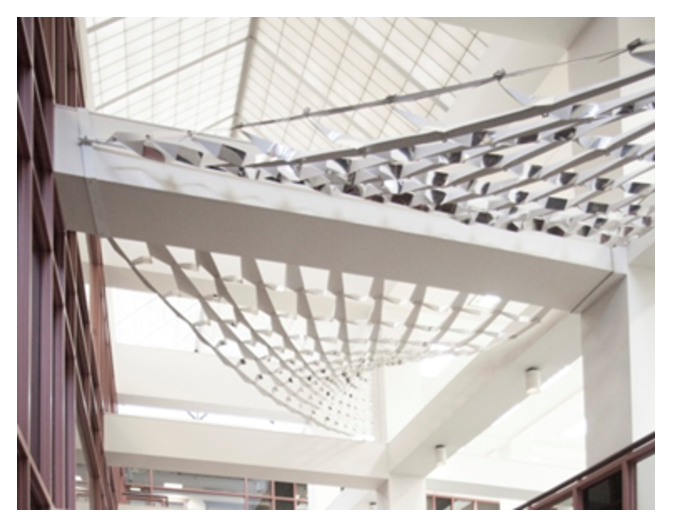
\includegraphics[width=0.5\linewidth]{figures/amp}
\label{fig:amp}}
\qquad \qquad
\subfloat[\mbox{ }]{
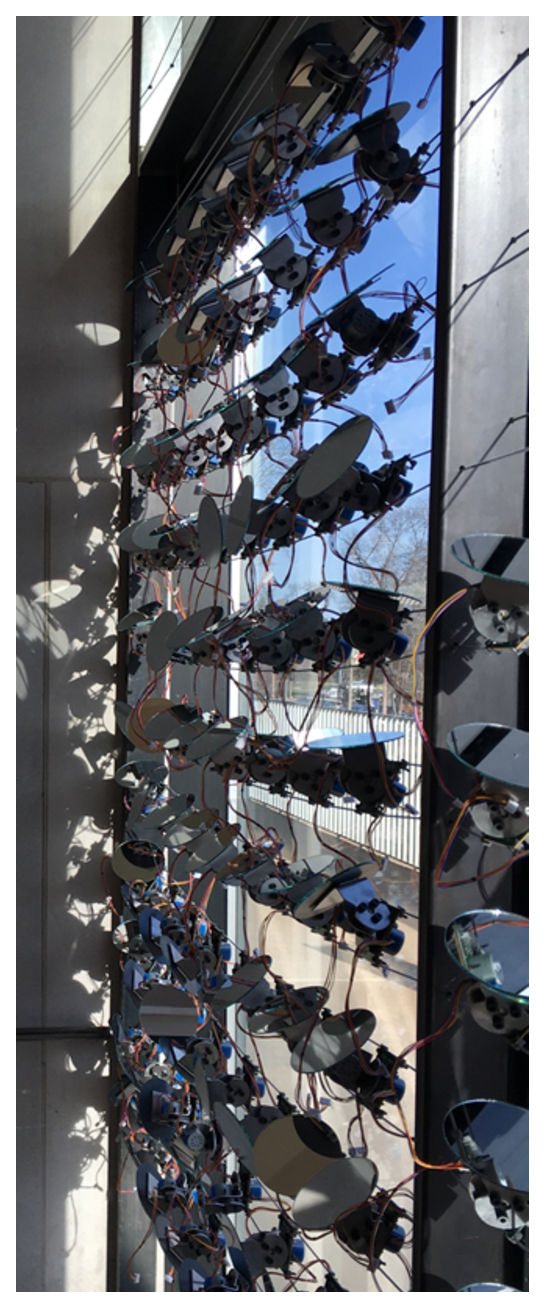
\includegraphics[width=0.16\linewidth]{figures/steinberg}
\label{fig:steinberg}}
\caption{Catoptric system prototypes.
(a)~\emph{AMP}, TRex building, St. Louis, MO.
(b)~\FIXME{name?}, Steinberg Hall, St. Louis, MO.
}
\label{fig:proto}
\end{figure}

In the next generation of this system, which is currently under construction,
over 600 mirrors are under active, 2-axis, microprocessor-based control and
therefore can be pointed in different directions dynamically as desired
over time. This installation is on the south wall of the Steinberg Hall
atrium (on
the campus of Washington University in St. Louis), and a subset of the
mirrors are shown in Figure~\ref{fig:steinberg}.

The ability to actively control the dynamic position of each mirror provides
for unprecidented capacity to position the available natural light where
it is desired.  This can easily change over time, as the usage of the
physical space changes.

The proposed research advances the investigation of reflected light by
designing specific intensities in some areas and dissipated lighting
conditions in other areas according to pre-determined, yet adjustable,
image-based maps. The maps can consist of any raster image and generate the
target positions for the reflected light in a space.  The image is sampled
according to intensity (black to white) to determine the density
of target points where the higher the value, the denser the resulting
field of points. Using an image-based map allows users to visualize
zones of intensity in an interior space prior to the mirrors reflecting
the daylight. Any user is capable of supplying or creating the image
to be used for the map, thus encouraging user control and interaction with
the system. The engagement of any member of a community on the creation
of that image has an impact on the entire community~\cite{BS13} and
encourages dialog about the quality and quantity of light within their
environment. 

Given the desire to control natural light (sunlight) via a catoptric surface,
repurposing it for illumination and/or thermal management, a number of
cruicial cyber-physical system issues must be addressed.
This research will investigate the following questions:
\begin{enumerate}

\item \emph{What are the qualitative and quantitative benefits
that can be achieved for bulding daylighting and thermal management
through the use of catoptric systems?}

Issues within this question include the ability to articulate the benefits
and to quantify them effectively.  Clearly, we are in the domain
of multi-objective control, so the relationship between the competing
goals must also be articulated and quantified. We intend to investigate
the use of Markov Decision Processes (MDPs) as an approach to
the multi-objective control problem, recognizing that maximization
(of an objective function) in expectation is a robust way to acknowledge
the inherent uncertainty of future events (whether it be sunlight availability,
lighting demand, or any other effect that is stochastic in nature).

\item \emph{How do we provide for the safety, reliability, maintainability, and
continued efficacy of these systems?}

Even with an ideal multi-objective control system in place, the system as
a whole has limited usefulness if these additional requirements are not
dealt with in an effective way.  Initially, just consider the issue of
safety: highly concentrated sunlight aimed at a heat collector (important
when harvesting energy for thermal management purposes) can be quite harmful
if inadvertently aimed at humans. 

Each of these system-level requirements must ultimately be included within
the optimization problem formulation, either as constraints (e.g., for
safety) or as additional objectives (e.g., reliability and/or maintainability).
Fortunately, the MDP formalism is well suited to the addition of concerns
such as these (especially those with a stochastic nature, as reliability
and maintainability tend to be).

\item \emph{Can we design abstractions that encapsulate subsystems for
effective reuse?}

A pair of immediate possibilities come to mind. Separating the concerns
of low-level control (e.g., of mirror positions) and high-level system
management (how the available light resource should be allocated) is one
option.  The low-level control subsystem can be encapsulated into a reusable
component, applicable to any number of physical positioning applications.
Similarly, a high-level management system (e.g., based upon MDP theory)
could also be encapsulated in a resuable component, applicable to any
number of other stochastic optimization problems.
Ultimately, we would like to generalize the above into abstractions that can be
leveraged more broadly for arbitrary cyber-physical systems development.

\end{enumerate}

\FIXME{Brief description of who we are and what we've done.}

\section{Background and Related Work}
\label{sec:background}

\FIXME{Describe first two installations.}

\begin{figure}[ht]
\centering
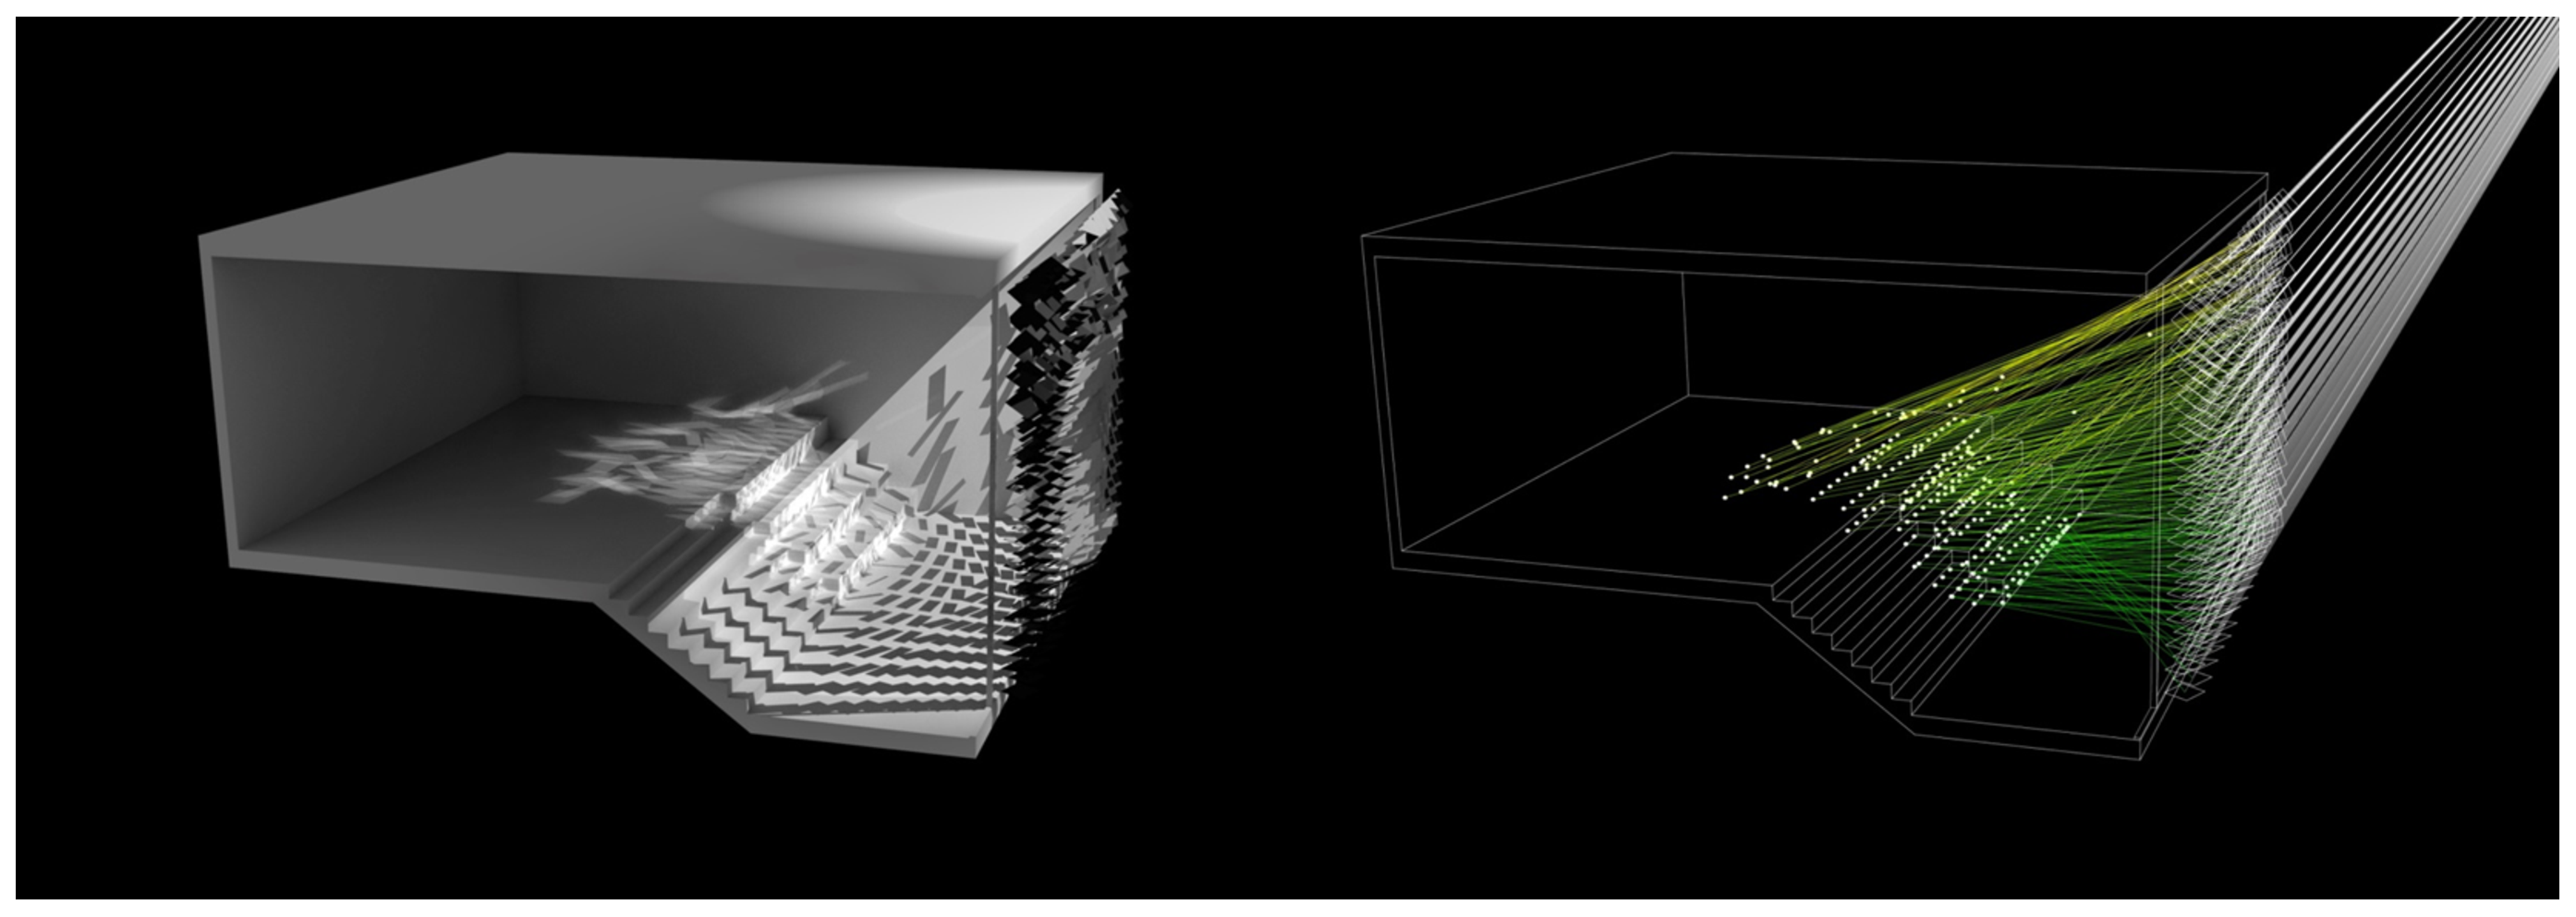
\includegraphics[width=0.8\linewidth]{figures/raytracing}
\label{fig:raytracing}
\caption{Ray tracing analysis of daylighting design.}
\end{figure}

Leslie~\cite{Leslie03} and Alrubaih et al.~\cite{azaise13} provide
a pair of review articles that effectively summarize the current
approaches to daylighting in modern building design.
For the most part, these are passive systems, or might include
active control of shades~\cite{kt16}, with a strong emphasis on
achieving uniform, homogeneous illumination~\cite{bwkk15,gb16}.
Our emphasis is on dynamic control of the light position, with the explicit
intent to be inhomogeneous in the illumination patterns.

There have been a number of efforts to quantitatively model and
empirically measure prototype daylighting
systems~\cite{bwkk15,fsdm14,ls06,vgf+13}. A pair of studies, first by
Lee and Selkowitz~\cite{ls06} and followed by Fernandes et al.\cite{fsdm14},
initially evaluated the potential for energy savings in the New York Times
Headquarters building and then measured the actual realized savings.

In this work, we will exploit Markov Decision Process (MDP)
formal theory~\cite{puterman} an an approach to optimization of the
catoptric surface control. MDPs represent a general approach
to modeling optimization problems and have been applied in a diverse set of
application areas~\cite{White93}. Examples include robotics~\cite{ab10}, 
economics~\cite{bs98}, experiment design~\cite{kb85},
medical decisions~\cite{ahsr10}, manufacturing~\cite{yyl04},
agriculture~\cite{Kristensen03},
and our own group's use in scheduling~\cite{gtsg08,tggs10}
and wireless spectrum management~\cite{mgc16}.

Our prior research has used Markov decision process
models~\cite{gtsg08} to generate resource management policies
off-line~\cite{gtgs09} for non-preemptive sharing of a resource
between multiple purposes at once on-line.  For example, a meter-tall robot's
camera (oriented by a pan-tilt unit similar to the ones we propose to
use in our multi-mirror catoptric installations) may be directed
downward to identify wire-frame chairs and other obstacles to
navigation that other sensors on the robot may have difficulty
detecting, or it may be directed upward to identify faces of people at
a reception whose images it can then capture. Given distributions of
the durations of intervals during which the camera would need to
remain pointed in a given direction to complete an individual task,
standard policy iteration techniques then can be used to generate
run-time policies that in expectation maximize an objective such as
adherence to a strictly proportional allocation of the resource over
time~\cite{gtsg08}, or even a more general definition of the utility 
of completing the different tasks at particular times~\cite{tggs10}.
We also showed that when different distributions of task completion
intervals can occur in different modes (e.g., when a robot moves
from room to room), it is possible to learn on-line what mode
the system is in, or if the mode is known what the distributions are,
but not both~\cite{gtgsuai10}.

However, policy iteration is exponentially expensive, and even the memory 
requirements to store complete policies for on-line use may be prohibitive 
in resource-limited systems.  We therefore focused next on the policies 
that were being generated from the models, and discovered consistent 
structure in those policies that allowed a reasonable heuristic 
approximation.  For simple proportional sharing, a single geometric partition
of a simplex could be calibrated to encode the appropriate policy accurately~\cite{gtspmgs10}.
For utility-based resource sharing multiple disjoint heuristics were needed but
the most effective one to use was clearly defined by problem parameters~\cite{tblwgs11}.

As a further illustration both of the applicability of MDP-based
policy iteration to generate effective resource management policies,
we applied similar techniques to manage a much different resource:
the transmission spectrum in wireless networks~\cite{mskgct13}.  Although 
the semantics of that resource differed radically from the pan-tilt camera, 
the MDP models were reasonably similar.  We extended the basic model to
include modulation as well as admission decisions, discovered and characterized
common structure among the policies that were generated, and again obtained
efficient and effective heuristic policies for on-line use~\cite{mgc16}.

In this proposal we adopt the definition used by Glaubius et al.~\cite{gtsg08}
of a (discrete-time) Markov decision process as a 5-tuple
$(\mathcal{X}, \mathcal{A}, T, R, \gamma)$, with \emph{states} designated
as $\chi \in \mathcal{X}$, \emph{actions} designated as $a \in \mathcal{A}$,
and a transition system, $T$, which gives the probability
$P_T (\chi' \mid \chi, a)$ of transitioning from state $\chi$ to
state $\chi'$ on action $a$.
The reward function $R(\chi, a, \chi') \in \mathbb R_{\ge 0}$ describes the
reward that accrues when transitioning from state $\chi$ to
state $\chi'$ via action $a$, under a discount factor, $\gamma$,
to ensure convergence of the long term reward.

\FIXME{Add transition into the next section.}

\section{Research Description}
\label{sec:research}

\subsection{Question 1 -- What are the qualitative and quantitative benefits
that can be achieved for building daylighting and thermal management
through the use of catoptric systems?}

There is ample literature that documents the benefits of natural light in
human-occupied spaces~\cite{Leslie03,ll01,pce00}, yet the thermal effects
can also be significant~\cite{bmbc13} (i.e., too much sunlight can
increase temperature to an unacceptable degree).

While many studies focus on the benefits of a homogeneous light levels
within a space~\cite{azaise13,bwkk15},
there is often differing need for light level based on user.
The increased control due to the independent positioning of the mirrors
can provide functional benefits for people that need more or less
light due to age of the occupant or their task. For example, someone using
a computer needs less light since the screen is a source of
artificial light while someone reading from physical media like
a book requires higher light levels. The light level required for
vision varies with the age of the occupants. As people get older,
they need higher light levels and increased luminous contrast.
Furthermore, everyone regardless of age have different qualities
of vision. Therefore, having a system that can accommodate these
varying conditions using daylight rather than artificial light is beneficial.

For thermal management, the literature on harvesting sunlight for space
heating is substantial (see, e.g.,~\cite{deW75,Hunt79,kbd76,Lunde80,smf08,wo06},
and we do not propose to contribute anything
new to that field.  We will simply leverage what are already well-understood
techniques. It is worth acknowledging that many sunlight-based heating systems
use catoptric systems (primarily for sun tracking). Our contributions here
will be to integrate a sunlight harvesting system into dual-purpose use, both
heating and illumination.

We will explore the use of Markov decision processes for multi-objective
control of catoptric systems.  We will start with a single objective,
matching a provided image map that represents a desired illumination pattern,
and then generalize to include the competing goal of thermal energy
harvesting.

For the purpose of designing an MDP, we will assume that a low-level
control mechanism exists that can position each individual mirror as
desired.  The MDP will model the higher-level management issues, e.g.,
which mirror should be pointed in which direction?
With a low-level controller in place, the state space, $\mathcal{X}$,
can encapsulate the set of mirrors pointed at each position in
the image map.  The set of actions, $\mathcal{A}$, will embody the movement
of one or more mirrors from their present position to a new position,
and the transition system, $T$, will encode the probabilistic variations
present in the available sunlight.  This allows the reward function, $R$,
to be a quantified match between the desired image map and the resulting
daylight that is directed to each position in the physical space.

After an initial exploration of the MDP formulated as described above,
we will then proceed to expand the framework to include the additional
objective of harvesting heat.  We will quantify the benefits of each
objective using general utility functions~\cite{tggs10} in a manner previously
explored by our group. One candidate set of utility functions we will
investigate will be to prioritize daylighting performance, and only
allocate excess sunlight to the HVAC subsystem. A second alternative
will be to proportionally provide sunlight to each goal up to the point
that the illumination can no longer benefit, at which point all additionally
available sunlight goes into heating.

In each of the above MDPs under investigation, we will utilize the
value-optimal solution (guaranteed to exist within Markov decision process
theory); however, this solution typically must be computed off-line, since
it is, in general, exponentially expensive to compute.  In parallel, we
will explore the space of value-optimal solutions and seek to formulate
an inexpensive to compute heuristic that closely approximates the
true value-optimal solution.

\subsection{Question 2 -- How do we provide for the safety, reliability,
maintainability, and continued efficacy of these systems?}

The ability to control mirror position is only useful over time if
the additional considerations of safety, reliability, etc., are managed
properly for the system as a whole. To address these issues, we will
investigate the degree to which they can be handled within the context
of the low-level controller versus being dealt with within the high-level
complete system control.

We anticipate some of these considerations being incorporated as constraints
within the optimization process and others as additional goals that we
wish to maximize during the multi-objective optimization itself.  Let us
first consider those that will be addressed as constraints (e.g., safety).

\paragraph{Constraints.}
A commonly used safety constraint on a positioning subsystem is to
specify hard limits on the range of motion (e.g., of each mirror, individually).
This kind of limit can be imposed by the physical design of the pan-tilt
mechanics, simply by adding physical stops at the limit positions.

The more interesting constraint systems occur when the safety considerations
are no longer locally determinable, but are dependent upon context.
An example that is relevant for our catoptric surfaces is a limit on
the total light intensity that can be supported at various positions in the
field of view of the mirrors. When providing heat into the HVAC system,
we desire a high light concentration delivered to the heat transfer point.
When illuminating a physical space for human occupants, the above
levels of light concentration are not only undesirable, they are patently
unsafe.

These context sensitive constraints add two additional requirements.
First, the higher-level management system must be responsible for them.
In our MDP formulation, we much adjust the feasible state space, $\mathcal{X}$,
so that they are unreachable (or have sufficiently negative reward as to
amount to the same thing).
Second, we must also ensure that whatever choices are made by the optimization
system (whether it be via MDPs or some other approach), the actual
mirror positions are still constrained so as to not result in an
unsafe condition.  This will require feedback of some form on the actual
mirror positions and the ability to determine whether or not the actual
positions differ from the controlled positions.  This might be accomplished
either locally (e.g., via shaft encoders on the pan-tilt mechanism) or
globally (e.g., via a visual monitoring system and appropriate image analysis
software).

\paragraph{Goals.}
Many of the additional considerations are more appropriately addressed as
additional (potentially competing) goals, adding to the desires of
daylighting and heating.  An example here would be the
impact on reliability of the system when individual mirrors are moved.  As
with all electro-mechanical systems, the pan-tilt mechanism has a limited
lifetime, which can be significantly impacted by its usage duty cycle
(i.e., the more it is moved, the sooner it will fail).

This is precisely the set of circumstances in which Markov decision
processes excel. \FIXME{defend this statement.}

\subsection{Question 3 -- Can we design abstractions that encapsulate
subsystems for effective reuse?}

\FIXME{We will investigate the viability and utility of two candidate
abstractions: direct mirror control and MDP control~\cite{cac18}.}

\subsection{Intellectual Merit}
\label{sec:merit}

The main intellectual contributions of this proposed research entail
the development of new methods for multi-objective optimization of 
catoptric systems, i.e., rigorous techniques for deciding how a 
collection of controllable mirrors should be installed and how they 
should be positioned and (repositioned) from moment to moment.  We
will investigate not only the multi-objective control models,
policies, and mechanisms, but also issues of design for flexible
installation; ensuring safety, reliability, etc.; and exploring in
what ways catoptric systems can serve as a guiding example for more
general cyber-physical systems development.  Conducting these 
investigations will provide new insights into how MDP models can
be applied in cyber-physical-human contexts, the benefits and limitations
of doing so, and practical experience developing, evaluating, and operating
these systems.

\section{Evaluation/Experimentation Plan}
\label{sec:eval}

We will organize our experimentation and evaluation activities around
three prototype catoptric surfaces.  The first is the system currently
being installed in the south window of Steinberg Hall's atrium (described
in Section~\ref{sec:background}).
The second will be designed for and installed at VelociData, Inc.,
a startup firm in
St.~Louis that is located in the recently announced \emph{39~North}
innovation district.
The third will be designed for an installed at BECS Technology, Inc.,
a local manufacturer of electronic control systems that has recently
relocated to a newly redeveloped 42,000~sq.~ft. facility. 
This is followed by a discussion of our software development
and assessment plans.

\subsection{Steinberg Hall, Washington University in St. Louis}

Steinberg Hall is situated on the Danforth Campus of Washington University
in St.~Louis. It is one of the buildings that houses the College
of Architecture, and is within easy walking distance of the Dept. of
Computer Science and Engineering.

The catoptric surface that is being installed at the south end of the
atrium will be complete by the start date of the proposed research project.
We will use it for a number of purposes:
\begin{enumerate}

\item Development and calibration of quantitative daylight delivery models.
We will evaluate the effectiveness of our current ray-tracing software
system in assessing the impact of different configurations of the surface
(i.e., various mirror positions).  Empirical evaluation will use a number
of light meters distributed within the space. The data collected will be
compared to our predictions as well as the analytical models
of both Bueno et al.~\cite{bwkk15} and Galatioto and Beccali~\cite{gb16}.

\item Practical aspects.
We will learn several practical things from this installation, including
the positioning precision achievable with our current physical design, the
viability of operating the mirror positioning motors open loop (the pan-tilt
is stepper motor driven and the current system does not incorporate
shaft encoders or other positioning feedback), the benefits (if any)
of controlling acceleration in addition to position, the timing
requirements for configuration changes, the ability to effect
multiple mirror movements in parallel, etc.

\item Investigation of the ability to provide positioning feedback via
image analysis.  We will install a camera with the full surface in its
field of view and assess the viability of using image analysis techniques
to discern the orientation of each mirror.  An imporant component of this
will be the degree of precision that is achievable.

\item Quantification of the viable heat transfer.
We will perform a controlled experiment in which we will focus varying
amounts of sunlight on a vessel of water to determine the temperature
rise that is achievable.  This will enable us to calibrate heat transfer
models that will go into the MDP formulation.

\item Reliability testing of the components.
This installation is not permanent. When it is decommissioned, we will
setup a representative collection of the mirror components in our laboratory
for stress testing (to failure).  This will allow us to calibrate our
reliability models for inclusion in the MDPs.

\end{enumerate}

\subsection{VelociData, Inc., 39 North Innovation District}

VelociData, Inc., is located at 10425 Old Olive Stree Rd., St.~Louis, MO.
They are in the \emph{39 North}
innovation district, which has the Danforth
Plant Science Center, Monsanto, Bio Research \& Development Growth Park,
and Heliz Center Biotech Incubator as anchors. It is a 10~min.~drive from
the Washington University Danforth Campus, and they have given us
permission to install a prototype at their facility (see letter
of collaboration).

There are a pair of potential installation sites at VelociData's location.
An east-facing window provides light to an individual's office, and
(the more interesting option) a pair of west-facing windows that provide
light to a bullpen of cubicles occupied by design engineers.

As we will not be able to tie into the HVAC system at this location, our
objectives will be focused on the daylighting benefits, including their
impact on the occupants of the space\footnote{All experimentation that
includes human subjects will undergo review by the Washington University
IRB prior to implementation.}.

We will use this installation for the following purposes:

\begin{enumerate}

\item Perform safety testing\footnote{Note: we only operate the Steinberg
surface under active human
supervision, as the automated safe operation cannot yet be ensured.}.
We will perform stess testing on the installed system, injecting errors so as to
intentionally attempt to create unsafe conditions, all the while monitoring
to ensure that safety is maintained.

\item Assess utility of non-southern facing windows.
Since the windows at VelociData's location are on the top floor, and face
either east or west, this gives us the opportunity to explore the viability
of exploiting multiple-reflection designs
(e.g., a fixed position mirror above the
roofline that redirects sunlight to the active catoptric surface).

\item Evaluate human response.
While we do not have the budget in this project to perform
comprehensive productivity analyses, we will be in a position to
query the building occupants about their experience with the
daylight effects. E.g., do they see value in the controllability
of the quantity of daylight?

\item Iterate the design.
As these are prototype systems, we have no expectation that the
initial versions will operate entirely as desired.  We will redesign
and rebuild as needed to make progress on the research questions we
are investigating.

\end{enumerate}

\subsection{BECS Technology, Inc., St. Louis County}

BECS Technology, Inc., is located at
10818~Midwest Industrial Dr., St.~Louis, MO.
They are a small manufacturer of electronic control
systems for a number of markets (e.g., agriculture, aquatics, refrigeration).
The unique benefit to this installation is that they have agreed to
allow us to have access to the HVAC system in their building (see letter
of collaboration).

The HVAC system at BECS is one in which the hydronic water loop
also serves as the fire protection sprinkler system~\cite{Janus01,wm79}.
Individual heat exchangers either deliver heat into the loop 
(e.g., from a boiler) or extract heat from the loop (e.g., to a
cooling tower).
An experimental loop that can be the focus point for light from
a catoptric surface is readily incorporated into a system such
as this.  The integration is made even easier because BECS, as
a manufacturer of aquatics equipment, uses a controller of its own
design to manage the entire system.

We will use this installation for the following purposes:

\begin{enumerate}

\item Repeat assessments from initial installations.
As each installation will have a unique configuration, we will exploit the
latter two installations (at VelociData and BECS) to perform common
experiments at each, comparing the results to increase the confidence
in any conclusions that we draw based on empirical data.
This will include all of the calibration efforts, as well as the comparison
of empirical data to the theoretical models (both for daylight delivery
and thermal heat transfer).
This will also include any human evaluations that are undertaken at
the VelociData site.

\item Integration into the HVAC system.
We will implement a heating loop that is capable of delivering
thermal energy into the building's main hydronic water loop.
The temperature of the water in this loop will be logged, and the
master HVAC controller (built by BECS) will enable us to determine
the effectiveness of the heat transfer.  We will also be able to
quantify the amount of energy savings that results.

\item Assessment of manufacturability.
As described in the Transfer to Practice Supplementary Document, BECS
is planning to assist us in evaluating the commercial viability of the
catoptric surface as a product.  An important piece of this evaluation is
the assessment (by design and manufacturing engineers at BECS) of the
manufacturability of the system.

\item Iterate the design. Again, we do not expect the initial design
to be all that it can be. As for the previous systems, we will redesign
and rebuild as needed.

\end{enumerate}

\subsection{Software Development and Assessment}

\FIXME{What should go here?}

\section{Project Management and Collaboration Plan}
\label{sec:collab}

We first describe the leadership team, including their primary roles
on the project.  This is followed by a description of our approach
to collaboration and a timeline for the research activities.

{\bf Roger D. Chamberlain}, PI, is Professor of Computer Science
and Engineering in the School of Engineering and Applied Science
at Washington University in St.~Louis.
Prof.~Chamberlain will have overall responsibility for managing the
research project and will take the lead in development of Markov
decision process models, performance evaluation, and electrical engineering
design requirements.

{\bf Chandler Ahrens}, Co-PI, is Asst.~Professor of Architecture
in the Sam Fox School of Design \& Visual Arts
at Washington University in St.~Louis.
Prof.~Ahrens will take the lead in the physical design aspects of
the catoptric surfaces, including their shape, configuration, positioning,
fabrication, and installation.

{\bf Chris D. Gill}, Co-PI, is Professor of Computer Science
and Engineering in the School of Engineering and Applied Science
at Washington University in St.~Louis.
Prof.~Gill will lead the software development efforts, with an emphasis
on designing for reuse whenever reasonable.  He will also lead our
approach to reusable abstractions that can be generalized to other
cyber-physical system uses.

All three faculty have worked together in the past, so the organization
of the present collaboration will be straightforward.  Co-authored
publications with two more of the faculty
include~\cite{cag18,mgc16, mskgct13}. Chamberlain and Ahrens collaborated
on the design and implementation of the catroptic surface being
installed in Steinberg Hall, and Chamberlain and Gill have previously
co-advised a doctoral student (J.~Meier, currently at Lockheed Martin)
who exploited Markov decision processes for RF spectrum management.

We will exploit the fact that the entire team is located on the
Danforth Campus of Washington University in St. Louis to organize
our collaboration around face-to-face meetings.  Our weekly meetings will
form the backbone of the collaboration, where we check in each other to
update status, plan next steps, and address any issues that have arisen
since our previous meeting.
We will also gather for the purpose of reviewing the literature
(traditional journal club activities), student presentations (frequently
practice talks for upcoming conference presentations), and reports
to the group from anyone who has recently returned from a conference trip.

Our initial plan for the project timeline is listed below, indicating the
primary activities to be pursued in each year of the project.

\subsection*{Year 1}

\begin{itemize}

\item Perform quantitative measurements on Steinberg catoptric surface.

\item Design initial MDPs, incorporating daylighting and heat harvesting.

\item Develop initial abstractions for low-level controller software.

\item Evaluate imaging approach for positioning feedback.

\item Perform initial design work for VelociData installation.

\item Submit human subjects evaluation plan to IRB for approval.

\end{itemize}

\subsection*{Year 2}

\begin{itemize}

\item Decommission Steinberg surface and re-purpose components for
reliability testing.

\item Expand MDPs to include additional constraints (i.e., to ensure
safety).

\item Develop initial abstractions for MDP-based optimization software.

\item Install VelociData catoptric surface and perform empirical evaluation.

\item Perform quality of experience evaluation for VelociData users.

\item Perform initial design work for BECS installation.

\end{itemize}

\subsection*{Year 3}

\begin{itemize}

\item Expand MDPs to include additional goals (e.g., to prioritize
reliability).

\item Install BECS catoptric surface and perform empirical evaluation.

\item Perform quality of experience evaluation for BECS users.

\item Refine software abstractions for both low-level positioning control
and high-level MDP-based optimization, based upon what has been learned
from earlier editions.

\item Release software under open source licensing terms.

\end{itemize}

\section{Broader Impacts}
\label{sec:broader}

The proposed research is expected to have important impacts on the built environment.
According to the EPA, buildings are responsible for producing 6\% of
greenhouse gasses and heat and electrical generation produces another
25\%\footnote{\url{https://www.epa.gov/ghgemissions/global-greenhouse-gas-emissions-data}}.
A large portion of the electrical consumption in buildings is used for
heating, cooling and artificial lighting. Our proposal addresses the
reduction of electricity for artificial lighting to be replaced by
reflected daylight and capturing the solar heat. During daytime hours,
daylight is a preferred source of light for many people and the proposal
directs the daylight deeper into a building. The daylight reflection system
provides a more sustainable approach by reducing the required electricity
and provides a more desirable quality of light.

At the undergraduate level, this work is closely related to
our second-semester introductory course in computer science and
computer engineering.  The
text (co-authored by PI R. Chamberlain) is entitled {\it Computing
in the Physical World}~\cite{cc17}, and the course provides an introduction to
cyber-physical systems concepts in a laboratory-based setting.

The computational platform used in the course (an Arduino Uno) is the
same one used to control the Steinberg prototype catoptric surface,
and it has a very large hobbyist following (in the maker community).
We regularly request support for Research Experience for Undergraduate
(REU) students, and individuals who have completed
the above course will be well prepared to contribute to the research.

At the graduate education level, this work will support 4 graduate
students at Washington Univ.~in St.~Louis.
These students will be some combination of engineering students and
architecture students, with each community of students learning from
the other to broaden their individual horizons of experience to
include multidisciplinary work.

The Steinberg prototype was substantially designed by a student pursuing
dual degrees in architecture (MArch) and engineering (MEng)~\cite{Mitchell18}.
He recently gave an invited presentation to the Washington University Board
of Trustees about his experience, and the university is considering
a broader set of educational offerings that are tailored to students with
similar, cross-disciplinary interests.

We will leverage a pair of existing university programs to help us
attract students from traditionally underrepresented groups.  The Olin
Fellowship Program (for women) and the Chancellor's Fellowship Program
(aimed to recruit, support, and retain underrepresented minority 
students) have a successful track
record of enabling individuals to pursue graduate study.  In our
experience, the most effective method for attracting students from
underrepresented groups is by personal contact with a suitable role
model.  To facilitate this, we regularly ask the appropriately
qualified individuals in our group to be actively involved in the
recruiting process.  This cohort currently includes two
minority graduate students (one African-American student and one Hispanic 
student).
We will attempt to leverage the maker space community as one target
for broadening participation from traditionally underrepresented groups.

\section{Results from Prior NSF Support}
\label{sec:prior}

\noindent
{\large\bf CSR: Small: Concurrent Accelerated Data Integration}
{\bf (CNS-1527510,
PI R. Chamberlain, co-PI Ron Cytron)}, 
10/2015--9/2019, \$519,275.  

\textbf{Intellectual Merit} -- This project investigates the
accelerated execution of data integration workflows, which
increasingly are bottlenecks in data science. Execution platforms
being targeted include both graphics engines and FPGAs.

\textbf{Broader Impacts} -- This research project has supported 3
graduate students and 4 REU students.  The applications investigated
come from the fields of computational biology, astrophysics, and the
Internet of Things, further expanding the scope of the students'
experience.

\textbf{Evidence of Research Products and their Availability} --
Publications resulting from this work include~\cite{dibs,c17,mgc16,js16}.
A benchmark suite of the above workflows has been released
as a community resource~\cite{dibsv1}.

\noindent
{\large\bf CPS: Medium: Collaborative: CyberMech, a Novel Run-Time Substrate for 
Cyber-Mechanical Systems}
{\bf (CNS-1136073 and CNS-1136075,
Washington University: PI C. Gill, co-PIs Kunal Agrawal and Chenyang Lu; Purdue University: PI Arun Prakash, co-PI Shirley Dyke)}, 9/2011-8/2016, \$1,800,000 total.  

This research project developed novel foundations for parallel real-time computing, and used them to demonstrate the first ever real-time hybrid simulation involving a thousand-degree-of-freedom structure.

\textbf{Intellectual Merit} -- Results of this research include new methods for parallel real-time execution of control and simulation computations, new parallel real-time scheduling techniques and analyses, and characterization and exploitation of trade-offs involving both high computational demand and stringent timing constraints.

\textbf{Broader Impacts} -- This multi-university project involved 7 PhD, 3 masters, and 7 undergraduate students, and 2 visiting scholars in highly multi-disciplinary research collaborations.  Results of this research appeared in 10 publications at top-tier conferences and journals.

\textbf{Evidence of Research Products and their Availability} -- Data, experiment configurations, platform software, and simulation source-code have been published on-line at Washington University and Purdue University.

\begin{comment}
\vspace{0.1in}
\noindent
{\large\bf Very Energetic Radiation Imaging Telescope Array (VERITAS) Project}
{\bf (J. Buckley)}

This work was covered by a combination of a DOE research grant as well
as project funds in the form of DOE and NSF/Physics subcontracts
through the Smithsonian Astrophysical Observatory project office.

\textbf{Intellectual Merit} -- Significant products of the
work include the VERITAS FADC electronics and a number of scientific
results summarized in
\cite{2016MNRAS.461..202A,2016arXiv160901692A,2016arXiv160806464A,2016arXiv160801569A,2016MNRAS.459.2550A,2016ApJ...821..129A,2016ApJ...819..156B,2016ApJ...818L..33A,2016ApJ...817L...7A,2015ApJ...815L..22A,2015PhRvL.115u1103C,2015PhRvD..91l9903A,2015A&A...578A..22A,2015A&A...576A.126A,2015PDU.....7...16B,2015ApJ...800...61A,2015ApJ...799....7A,2014ApJ...797...89A,2014ApJ...795L...3A,2014ApJ...790..149A,2014ApJ...788..158A,2014ApJ...788...78A,2014ApJ...787..166A,2014ApJ...783...16A,2014ApJ...782...13A,2014APh....54....1A,2014arXiv1401.6085F,2014ApJ...780..168A,2013ApJ...779...92A,2013arXiv1310.8621A,2013arXiv1310.7040B,2013arXiv1310.5662B,2013ApJ...776...69A,2013arXiv1308.6173V,2013arXiv1307.4962P,2013arXiv1307.2807D,2013ApJ...770...93A,2013arXiv1305.0302W,2013arXiv1304.6367S,2013APh....43....3A,2013ApJ...764...38A,2013ApJ...762...92A}.
A founding member of VERITAS, Dr.\ Buckley was responsible for the design
and construction of the 2000-channel 500 Msps VERITAS FADC system.
He also played a leading role in establishing the scientific
programs for dark matter, multiwavelength studies of active galaxies
and observations of supernova remnants. Scientific highlights of
VERITAS include (1) DM limits on dwarf
galaxies\cite{2017PhRvD..95h2001A,2015PhRvD..91l9903A,2012PhRvD..85f2001A},
(2) resolved images and spectra from supernova remnants (SNR) leading
to direct evidence for the origin of hadronic cosmic rays in SNR
\cite{2017ApJ...836...23A,2013ApJ...764...38A,2013ApJ...770...93A,2010ApJ...719L..69A,2009ApJ...698L.133A},
(3) discovery of periodic emission from the Crab pulsar up to $>$100
GeV challenging current models of pulsar magnetospheres
\cite{2011Sci...334...69V}), (4) measurements of spectral variability
of active galaxies (AGNs) with multiwavelength data providing new
constraints on conditions near the central supermassive black hole
(e.g.,
\cite{2009ApJ...707..612A,2008ApJ...684L..73A,2011ApJ...726...43A,2009ApJ...691L..13D,2017ApJ...834....2A})
and (5) constraints on the extragalactic background light,
Lorentz-invariance violation and intergalactic magnetic fields
\cite{2012ApJ...750...94A,2010ApJ...708L.100A}.

\textbf{Broader Impacts} -- Information on VERITAS was disseminated to the
general public through YouTube videos, public site tours, and informational
displays at the Smithsonian Astrophysical Observatories. 

\textbf{Evidence of Research Products and their Availability} --

\end{comment}

%\input{conclude}

\clearpage
% \begin{scriptsize}
\bibliographystyle{abbrv}
%\bibliography{prop,wu,astro,refs}
\bibliography{prop}
% \end{scriptsize}

\end{document}
